\subsection{A heliocentrikus modell "újrafelfedezése"}

\begin{frame}{}
    \centering
    \Huge{Heliocentrikus modell "újrafelfedezése"}\\
    \vspace*{1cm}
    \large{}
\end{frame}

\begin{frame}{Fizikai modellek tanulása 1.}
    \centering
    \begin{tikzpicture}
        \draw[rounded corners,draw=dblue,fill=dblue!40] (-0.5,-1.2) rectangle (2.5,1.5);
        \draw[rounded corners,draw=lorange,fill=lorange!40] (3.5,-0.5) rectangle (5,0.5);
        \draw[rounded corners,draw=dblue,fill=dblue!40] (5.9,-0.5) rectangle (8.7,0.5);
        \draw[rounded corners,draw=dblue,fill=dblue!40] (3.9,1.5) rectangle (4.5,2.5);
        
        \draw [->] (0,-1) -- (0,1);
        \draw [->] (0,0) -- (2,0);
        \draw [dashed] (0,-0.5) -- (1.5,0.5);
        \draw (1,-1.5) node {\small Megfigyelés};
        \draw (2.2,0) node {\footnotesize t};
        \draw (0,1.2) node {\footnotesize x};
        
        \draw (3,0) node {$\Longrightarrow$};
        
        \draw (4.2,0.2) node {$x_0 = \_$};
        \draw (4.2,-0.2) node {$v = \_$};
        \draw (4.2,-1) node {Reprezentáció};
        
        \draw (5.5, 0) node {$\Longrightarrow$};
        
        \draw (7.3,0) node {$x(t') = x_0 + vt'$};
        \draw (7.3,-1) node {Válasz};
        
        \draw (4.2,2) node {$t'$};
        \draw (4.2,1.2) node {Kérdés};
        \draw[->] (4.6,2) -- (5.5,0.2);
        
        
        \draw (3,-2) node {Encoding};
        \draw (5.5,-2) node {Decoding};
        \draw[->,dashed] (3,-1.8) -- (3,-0.2);
        \draw[->,dashed] (5.5,-1.8) -- (5.5, -0.2);
    \end{tikzpicture}
\end{frame}

\begin{frame}{Autoencoder}
    \centering
    \begin{tikzpicture}
        \foreach \y in {-3,-2,-1,0,1,2,3} {
            \draw[draw=dblue!50,fill=dblue!50] (-3, \y) circle [radius=0.4cm];
            \draw[draw=dblue!50,fill=dblue!50] (5, \y) circle [radius=0.4cm];
            \draw[->] (-4, \y) -- (-3.4, \y);
            \draw[->] (5.4, \y) -- (6, \y);
            
            \foreach \yy in {-2,-1,0,1,2} {
                \draw[->] (-2.6, \y) -- (-1.4, \yy);
                \draw[->] (3.4, \yy) -- (4.6, \y);
            }
        }
        
        \foreach \y in {-2,-1,0,1,2} {
            \draw[draw=dblue!50,fill=dblue!50] (-1, \y) circle [radius=0.4cm];
            \draw[draw=dblue!50,fill=dblue!50] (3, \y) circle [radius=0.4cm];
            
            \foreach \yy in {-1,0,1} {
                \draw[->] (-0.6, \y) -- (0.6, \yy);
                \draw[->] (1.4, \yy) -- (2.6, \y);
            }
        }
        
        \foreach \y in {-1,0,1} {
            \draw[draw=orange!50,fill=orange!50] (1, \y) circle [radius=0.4cm];
        }
        
        \draw[dashed] (0, 3.5) -- (0, -3.5);
        \draw[dashed] (2, 3.5) -- (2, -3.5);
        \draw (-1.5, 3) node {Encoder};
        \draw (3.5,3) node {Decoder};
        \draw (1,3) node {Reprezentáció};
    \end{tikzpicture}
\end{frame}

\begin{frame}{Fizikai modellek tanulása 2.}
    \centering
    \begin{tikzpicture}[scale=0.9]
        \foreach \y in {-1,0,1} {
            \draw[draw=lblue!50,fill=lblue!50] (-5,\y) circle [radius=0.4cm];
            \foreach \yy in {-2,-1,0,1,2} {
                \draw[->] (-4.6, \y) -- (-3.4, \yy);
            }
        }
        
        \foreach \y in {-2,-1,0,1,2} {
            \foreach \x in {-3,-1,3,5} {
                \draw[draw=dblue!50,fill=dblue!50] (\x, \y) circle [radius=0.4cm];
            }
        }
        
        \foreach \y in {-0.5,0.5} {
            \draw[draw=lorange!50,fill=lorange!50] (1,\y) circle [radius=0.4cm];
            \foreach \yy in {-2,-1,0,1,2} {
                \draw[->] (-0.6, \yy) -- (0.6, \y);
                \draw[->] (1.4, \y) -- (2.6, \yy);
            }
        }
        
        \foreach \y in {-2,-1,0,1,2} {
            \foreach \yy in {-2,-1,0,1,2} {
                \draw[->] (-2.6, \y) -- (-1.4, \yy);
                \draw[->] (3.4, \y) -- (4.6, \yy);
            }
            \draw[->] (5.4, \y) -- (6.6,0);
        }
        \draw[draw=lblue!50,fill=lblue!50] (7,0) circle [radius=0.4cm];
        \draw[draw=lblue!50,fill=lblue!50] (1,4) circle [radius=0.4cm];
        
        \foreach \y in {-2,-1,0,1,2} {
            \draw[->] (1.2, 3.7) -- (2.6, \y);
        }
        
        \draw (-2,-3) node {\small Encoder};
        \draw (4,-3) node {\small Decoder};
        \draw (-5,2) node {\small Megfigyelés};
        \draw (1,-1.5) node {\small Reprezentáció};
        \draw (7,-1) node {\small Válasz};
        \draw (0,4) node {\small Kérdés};
    \end{tikzpicture}
\end{frame}

\begin{frame}{Autoencoder - Kerék meghibásodás}
    \centering
    \includegraphics[width=1.0\textwidth]{figures/gear_measurements.png}
\end{frame}

\begin{frame}{Autoencoder - Kerék meghibásodás}
    \centering
    \includegraphics[width=1.0\textwidth]{figures/gear_rec_loss.png}
\end{frame}


\begin{frame}{Heliocentrikus modell "újrafelfedezése"}
    \centering
    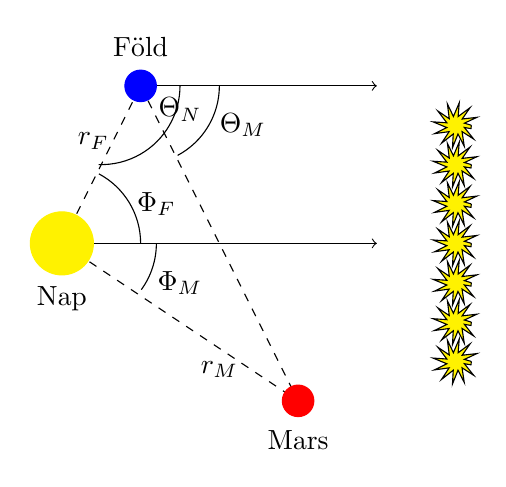
\begin{tikzpicture}
        \draw[dashed] (0,0) -- (1,2)
                      (0,0) -- (3,-2)
                      (1,2) -- (3,-2);
        \draw[->] (0,0) -- (4,0);
        \draw[->] (1,2) -- (4,2);
        
        \draw (1,0cm)   arc (0:62:1cm);
        \draw (1.2,0cm) arc (0:-36:1cm);
        \draw (2,2)   arc (0:-62:1cm);
        \draw (1.5,2)   arc (0:-92:1cm);
        
        \foreach \y in {-1.5,-1,-0.5,0,0.5,1,1.5} {
            \draw [fill=yellow,decorate,decoration={zigzag,segment length=3}] (5,\y) circle (0.2cm);
        }
        
        \draw[fill=yellow,draw=yellow] (0,0) circle (0.4cm);
        \draw[fill=blue,draw=blue]     (1,2) circle (0.2cm);
        \draw[fill=red,draw=red]       (3,-2) circle (0.2cm);
        
        \draw (0,-0.7) node {Nap}
              (3,-2.5) node {Mars}
              (1,2.5) node {Föld}
              (2,-1.6) node {$r_M$}
              (0.4,1.3) node {$r_F$}
              (1.2,0.5) node {$\Phi_F$}
              (1.5,-0.5) node {$\Phi_M$}
              (1.5, 1.7) node {$\Theta_N$}
              (2.3, 1.5) node {$\Theta_M$};
    \end{tikzpicture}
\end{frame}

\begin{frame}{Heliocentrikus modell "újrafelfedezése"}
    \centering
    \begin{tikzpicture}
        \foreach \y in {-0.5,0,0.5} {
            \draw[fill=lblue!50,draw=lblue!50] (0, \y) circle (0.2cm);
            \foreach \yy in {-1,-0.5,0,0.5,1} {
                \draw[->] (0.2,\y) -- (0.8, \yy);
            }
        }
        
        \foreach \y in {-1,-0.5,0,0.5,1} {
            \foreach \x in {1,2} {
                \draw[fill=dblue!50,draw=dblue!50] (\x, \y) circle (0.2cm);
            }
            \foreach \yy in {-1,-0.5,0,0.5,1} {
                \draw[->] (1.2, \y) -- (1.8, \yy);
            }
        }
        
        \foreach \y in {-0.25,0.25} {
            \draw[fill=lorange!50,draw=lorange!50] (3, \y) circle (0.2cm);
            \foreach \x in {4,5,7,8} {
                \draw[fill=dblue!50,draw=dblue!50] (\x, \y) circle (0.2cm);
            }
            \foreach \yy in {-1,-0.5,0,0.5,1} {
                \draw[->] (2.2, \yy) -- (2.8, \y);
            }
        }
        
        \foreach \x in {3,4,5,6,7,8,9} {
            \foreach \y in {-0.25,0.25} {
                \foreach \yy in {-0.25,0.25} {
                    \draw[->] (\x+0.2, \y) -- (\x+0.8, \yy);
                }
            }
        }
        
        \foreach \x in {6, 9} {
            \foreach \xx in {\x-1,\x-0.5,\x,\x+0.5,\x+1} {
                \foreach \y in {-0.25,0.25} {
                    \draw[fill=lorange!50,draw=lorange!50] (\x, \y) circle (0.2cm);
                    \draw[->] (\x, \y+0.2) -- (\xx, 1.8);
                }
                \draw[fill=dblue!50,draw=dblue!50] (\xx, 2) circle (0.2cm);
                \draw[fill=dblue!50,draw=dblue!50] (\xx, 3) circle (0.2cm);
                \foreach \xxx in {\x-1,\x-0.5,\x,\x+0.5,\x+1} {
                    \draw[->] (\xx, 2.2) -- (\xxx, 2.8);
                }
                \foreach \xxx in {\x-0.25,\x+0.25} {
                    \draw[->] (\xx, 3.2) -- (\xxx, 3.8);
                }
            }
            \foreach \xx in {\x-0.25,\x+0.25} {
                \draw[fill=lblue!50,draw=lblue!50] (\xx, 4) circle (0.2cm);
            }
        }
        
        \draw (-0.5,1) node {\footnotesize Megfigyelés};
        \draw (1.5,-1.5) node {\footnotesize Encoder};
        \draw (3, -1) node {\footnotesize $r(t_0)$};
        \draw (6, -1) node {\footnotesize $r(t_1)$};
        \draw (9, -1) node {\footnotesize $r(t_2)$};
        \draw (4.5, -1) node {\footnotesize Időlépés};
        \draw (7.5, -1) node {\footnotesize Időlépés};
        \draw (4, 2.5) node {\footnotesize Decoder};
        \draw (4.5, 4) node {\footnotesize Válasz};
    \end{tikzpicture}
\end{frame}

\begin{frame}{Heliocentrikus modell "újrafelfedezése"}

    {\bf Probléma}: $\Theta_M(t)$ és $\Theta_N(t)$ előrejelzése a Földről nézve, ha ismert $\Theta_M(t_0)$ és $\Theta_N(t_0)$. \\
    {\bf Fizikai modell}: A bolygók körpályán keringenek a Nap körül egyenletes sebességgel (adatgenerálás miatt). \\
    {\bf Megfigyelés}: $(\Theta_M(t_0), \Theta_N(t_0))$ párosok (ez a neurális háló bemente) \\
    {\bf Kérdés}: Implicit \\
    {\bf Válasz}: Szögmérések sorozata $(\Theta_M(t_1), \Theta_N(t_1)), \dots, (\Theta_M(t_n), \Theta_N(t_n))$ \\
    {\bf Főbb eredmények}:
        \begin{itemize}
            \item $\Phi_F$ és $\Phi_M$ szögek tárolása ahogy a Naptól látszódik
            \item 0.4\%-os hibával becsüli a szögeket
        \end{itemize}
\end{frame}
